% ARPEGOS:  Automatized Roleplaying-game Profile Extensible Generator Ontology based System %
% Author : Alejandro Muñoz Del Álamo %
% Copyright 2019 %

% Section 4.2: Modelo de Casos de Uso %
\section{Modelo de Casos de Uso}
Ahora que se dispone de una estructura clara para el diseño de ontologías del sistema, hay que 
explicar cómo se resuelven los diferentes requisitos funcionales comentados en el apartado 
\ref{Requisitos_funcionales}. Por esa razón, en este apartado se mostrarán los diferentes 
\textit{casos de uso} del sistema, que, como plantea Cockburn \autocite*{Cockburn2000}, 
describen las diferentes interacciones posibles entre los actores y el sistema asociadas a una meta concreta. \medskip

\subsection{Actores}
En este sistema no se aprecia diferencia alguna entre usuarios, por lo que todos ellos se consideran como un único 
agente externo, disponiendo todos ellos de los mismos privilegios.

\begin{table}[H]
    \centering
    \begin{tabular}{|c|c|}
        \hline
        \thead{\textit{\textbf{Actor}}} & \thead{\textit{\textbf{Descripción}}} \\ \hline \hline
        \makecell{\textbf{Usuario}} & \makecell{Es la persona que interacciona con la aplicación, \\ haciendo uso de las funciones que esta posee.} \\ \hline
    \end{tabular}
    \caption{Tabla de actores}
    \label{Tabla_actores}
\end{table}

\subsection{Descripción de casos de uso}

Inicialmente, se va a describir un caso de uso de alto nivel que representa todos los requisitos del sistema que 
requieren algún tipo de interacción por parte del usuario. \medskip

\begin{figure}[H]
    \centering
    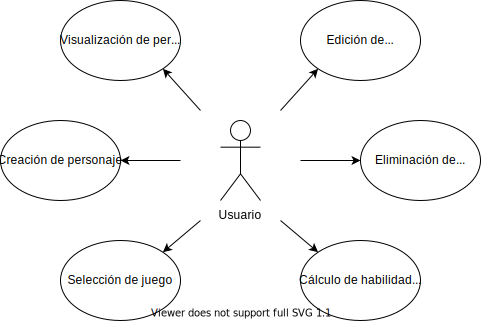
\includegraphics[scale=0.7]{Documentation-Scheme/Desarrollo/Análisis-Sistema/Modelo-Casos-Uso.pdf}
    \caption{Diagrama de Casos de Uso del sistema}
    \label{Caso_uso_sistema}    
\end{figure}

Como en la mayoría de casos de uso es necesario conocer el juego que se va a utilizar, se va a considerar que en los casos 
que no estén directamente relacionados con la gestión de juegos, el primer paso es \textit{Seleccionar juego}, para simplificar 
los diagramas y facilitar su comprensión.

\subsection{Gestión de juegos}

\begin{figure}[H]
    \centering
    \includegraphics[scale=0.7]{Documentation-Scheme/Desarrollo/Análisis-Sistema/Caso_Uso_Juegos.pdf}
    \caption{Diagrama de Casos de Uso: Gestión de juegos}
    \label{Diagrama_gestión_juegos}    
\end{figure}


\subsubsection{Caso de uso: Añadir juego} 
\begin{itemize}
    \item \textbf{Descripción}: El usuario añade un juego o una versión de un juego a la aplicación.
    \item \textbf{Precondiciones}: El usuario debe disponer del fichero de información del juego en el 
    dispositivo que contiene la aplicación.
    \item \textbf{Postcondiciones}: La aplicación tiene acceso a un nuevo juego.
\end{itemize}

\paragraph{\textit{Identificación de escenarios}}
\subparagraph{Escenario principal}
\begin{enumerate}
    \item El usuario desea introducir un nuevo juego en la aplicación.
    \item El usuario pulsa el botón de \textit{Añadir juego}.
    \item El usuario selecciona la opción \textit{Juego nuevo}.
    \item El usuario introduce el nombre del juego.
    \item El usuario indica el fichero de información del juego.
    \item El usuario pulsa el botón de \textit{Aceptar}.
    \item El sistema crea la estructura de carpetas para el nuevo juego.
    \item El sistema copia el fichero en su nueva ubicación, de manera que ya está listo 
    para su uso en el sistema.
\end{enumerate}

\subparagraph{Escenario alternativo: Añadir nueva versión de un juego ya existente}
\begin{enumerate}
    \item El usuario desea introducir un nuevo juego en la aplicación.
    \item El usuario pulsa el botón de \textit{Añadir juego}.
    \item El usuario selecciona la opción \textit{Actualizar juego}.
    \item El usuario indica el directorio en el que debe ubicarse el juego que desea incluir.
    \item El usuario indica el fichero de información del juego.
    \item El usuario pulsa el botón de \textit{Aceptar}.
    \item El sistema copia el fichero en su nueva ubicación, de manera que ya está listo 
    para su uso en el sistema.
\end{enumerate}

\subsubsection{Caso de uso: Seleccionar juego}
\begin{itemize}
    \item \textbf{Descripción}: El usuario elige un juego disponible en la aplicación.
    \item \textbf{Precondiciones}: El usuario debe disponer de algún juego en la aplicación.
    \item \textbf{Postcondiciones}: La aplicación toma el juego y la versión indicados
    como juego y versión activos hasta que se realice una nueva selección.
\end{itemize}

\paragraph{\textit{Identificación de escenarios}}
\subparagraph{Escenario principal}
\begin{enumerate}
    \item El usuario desea seleccionar un juego de la aplicación.
    \item El usuario pulsa el botón de \textit{Seleccionar juego}.
    \item El sistema muestra un listado con los juegos disponibles.
    \item El usuario selecciona una de las opciones mostradas.
    \item El sistema muestra todas las versiones disponibles del juego seleccionado.
    \item El usuario selecciona una de las opciones mostradas.
    \item El usuario pulsa el botón de \textit{Aceptar}.
    \item El sistema crea la estructura de carpetas para el nuevo juego.
    \item El sistema copia el fichero en su nueva ubicación, de manera que ya está listo 
    para su uso en el sistema.
\end{enumerate}

\subsubsection{Caso de uso: Eliminar juego}
\begin{itemize}
    \item \textbf{Descripción}: El usuario elimina un juego disponible de la aplicación.
    \item \textbf{Precondiciones}: El usuario debe disponer de algún juego en la aplicación.
    \item \textbf{Postcondiciones}: La aplicación elimina toda la información relacionada 
    con el juego en cuestión.
\end{itemize}

\newpage
\paragraph{\textit{Identificación de escenarios}}
\subparagraph{Escenario principal}
\begin{enumerate}
    \item El usuario desea eliminar un juego de la aplicación.
    \item El usuario pulsa el botón de \textit{Eliminar juego}.
    \item El usuario selecciona la opción de \textit{Eliminar juego completo}.
    \item El sistema muestra un listado con los juegos disponibles.
    \item El usuario selecciona una de las opciones mostradas.
    \item El sistema realiza una pregunta de confirmación.
    \item El usuario pulsa la opción \textit{Eliminar}.
    \item El sistema elimina todos los elementos relacionados con el juego seleccionado.
\end{enumerate}

\subparagraph{Escenario alternativo: Eliminar una versión de un juego sin eliminar el juego completo}
\begin{enumerate}
    \item El usuario desea eliminar un juego de la aplicación.
    \item El usuario pulsa el botón de \textit{Eliminar juego}.
    \item El usuario \textbf{no} selecciona la opción de \textit{Eliminar juego completo}.
    \item El sistema muestra un listado con los juegos disponibles.
    \item El usuario selecciona una de las opciones mostradas.
    \item El sistema muestra todas las versiones disponibles del juego seleccionado.
    \item El usuario selecciona una de las opciones mostradas.
    \item El usuario pulsa el botón \textit{Aceptar}.
    \item El sistema realiza una pregunta de confirmación.
    \item El usuario pulsa la opción \textit{Eliminar}.
    \item El sistema elimina la versión indicada del juego seleccionado.
\end{enumerate}

\newpage
\subsection{Gestión de personajes}
\begin{figure}[H]
    \centering
    \includegraphics[scale=0.7]{Documentation-Scheme/Desarrollo/Análisis-Sistema/Caso_Uso_Personajes.pdf}
    \caption{Diagrama de Casos de Uso: Gestión de personajes}
    \label{Diagrama_gestión_personajes}    
\end{figure}

\subsubsection{Caso de uso: Crear personaje}
\begin{itemize}
    \item \textbf{Descripción}: El usuario crea un personaje siguiendo las normas del juego y la versión activos.
    \item \textbf{Precondiciones}: El usuario debe haber seleccionado el juego deseado previamente.
    \item \textbf{Postcondiciones}: La aplicación genera un fichero con la información del personaje 
    y lo almacena en la carpeta de personajes correspondiente al juego activo.
\end{itemize}

\paragraph{\textit{Identificación de escenarios}}
\subparagraph{Escenario principal}
\begin{enumerate}
    \item El usuario desea crear un personaje del juego activo en la aplicación.
    \item El usuario pulsa el botón de \textit{Crear personaje}.
    \item El usuario introduce el nombre del personaje.
    \item El sistema muestra las diversas etapas de creación del personaje correspondiente del juego, presentadas 
    a modo de carrusel, de manera que permite al usuario avanzar y retroceder de etapa según lo necesite.
    \item El usuario configura el personaje a su medida.
    \item El usuario presiona el botón \textit{Finalizar} una vez ha terminado de configurar el personaje.
    \item El sistema genera el fichero del personaje y lo almacena en la carpeta de personajes del juego correspondiente.
\end{enumerate}

\subsubsection{Caso de uso: Visualizar personaje}
\begin{itemize}
    \item \textbf{Descripción}: El usuario visualiza un personaje del juego activos.
    \item \textbf{Precondiciones}: El personaje debe haber sido creado previamente.
    \item \textbf{Postcondiciones}: La aplicación muestra la información del personaje.
\end{itemize}

\paragraph{\textit{Identificación de escenarios}}
\subparagraph{Escenario principal}
\begin{enumerate}
    \item El usuario desea visualizar la información de un personaje del juego activo en la aplicación.
    \item El usuario pulsa el botón de \textit{Visualizar personaje}.
    \item El sistema muestra el listado de personajes del juego activo.
    \item El usuario selecciona una de las opciones mostradas.
    \item El sistema muestra la información del usuario, separada por etapas a modo de carrusel, de manera 
    que permite al usuario navegar entre etapas según lo necesite.
\end{enumerate}

\subparagraph{Escenario alternativo: Editar información del personaje}
\begin{enumerate}
    \item Este escenario se describe en el caso de uso \textit{Editar personaje}.
\end{enumerate}

\subparagraph{Escenario alternativo: Eliminar personaje}
\begin{enumerate}
    \item Este escenario se describe en el caso de uso \textit{Eliminar personaje}.
\end{enumerate}

\subsubsection{Caso de uso: Editar personaje}
\begin{itemize}
    \item \textbf{Descripción}: El usuario modifica información de un personaje del juego activo.
    \item \textbf{Precondiciones}: El personaje debe haber sido creado previamente.
    \item \textbf{Postcondiciones}: La aplicación sobreescribe la información del personaje.
\end{itemize}

\newpage
\paragraph{\textit{Identificación de escenarios}}
\subparagraph{Escenario principal}
\begin{enumerate}
    \item El usuario desea visualizar la información de un personaje del juego activo en la aplicación.
    \item El usuario pulsa el botón de \textit{Visualizar personaje}.
    \item El sistema muestra el listado de personajes del juego activo.
    \item El usuario selecciona una de las opciones mostradas.
    \item El sistema muestra la información del usuario, separada por etapas a modo de carrusel, de manera 
    que permite al usuario navegar entre etapas según lo necesite.
    \item El usuario pulsa el botón de \textit{Editar información de etapa}.
    \item El sistema muestra la vista de edición de la etapa en cuestión.
    \item El usuario altera en parte o en su totalidad el contenido de la vista.
    \item El usuario pulsa el botón \textit{Guardar cambios}
    \item El sistema realiza una pregunta de seguridad.
    \item El usuario pulsa el botón \textit{Guardar}.
    \item El sistema sobreescribe el fichero del personaje con los nuevos valores.
\end{enumerate}

\subsubsection{Caso de uso: Eliminar personaje}
\begin{itemize}
    \item \textbf{Descripción}: El usuario elimina un personaje del juego activo.
    \item \textbf{Precondiciones}: El personaje debe haber sido creado previamente.
    \item \textbf{Postcondiciones}: La aplicación sobreescribe la información del personaje.
\end{itemize}

\paragraph{\textit{Identificación de escenarios}}
\subparagraph{Escenario principal}
\begin{enumerate}
    \item El usuario desea visualizar la información de un personaje del juego activo en la aplicación.
    \item El usuario pulsa el botón de \textit{Visualizar personaje}.
    \item El sistema muestra el listado de personajes del juego activo.
    \item El usuario selecciona una de las opciones mostradas.
    \item El sistema muestra la información del usuario, separada por etapas a modo de carrusel, de manera 
    que permite al usuario navegar entre etapas según lo necesite.
    \item El usuario pulsa el botón de \textit{Eliminar personaje}.
    \item El sistema realiza una pregunta de seguridad.
    \item El usuario pulsa el botón \textit{Eliminar}.
    \item El sistema elimina el fichero del personaje.
\end{enumerate}

\subsection{Gestión de habilidades}
\begin{figure}[H]
    \centering
    \includegraphics[scale=0.7]{Documentation-Scheme/Desarrollo/Análisis-Sistema/Caso_Uso_Habilidades.pdf}
    \caption{Diagrama de Casos de Uso: Gestión de habilidades}
    \label{Diagrama_gestión_habilidades}    
\end{figure}

\subsubsection{Caso de uso: Calcular habilidad}
\begin{itemize}
    \item \textbf{Descripción}: El usuario conocer el resultado de una habilidad aplicando los modificadores 
    correspondientes al resultado del lanzamiento de dados.
    \item \textbf{Precondiciones}: El personaje debe haber sido creado previamente.
    \item \textbf{Postcondiciones}: La aplicación calcula el valor final de la habilidad aplicando los 
    modificadores almacenados en el fichero del personaje.
\end{itemize}

\paragraph{\textit{Identificación de escenarios}}
\subparagraph{Escenario principal}
\begin{enumerate}
    \item El usuario desea calcular el resultado de una habilidad de un personaje.
    \item El usuario pulsa el botón de \textit{Calcular habilidad de personaje}.
    \item El sistema muestra la pantalla de cálculo de habilidades.
    \item El usuario pulsa el botón de \textit{Seleccionar personaje}.
    \item El sistema muestra el listado de personajes del juego activo.
    \item El usuario selecciona una de las opciones mostradas.
    \item El usuario pulsa el botón de \textit{Seleccionar habilidad}.
    \item El sistema muestra un listado con las habilidades disponibles del personaje.
    \item El usuario selecciona una de las opciones mostradas.
    \item El usuario introduce el valor del lanzamiento de dados.
    \item El usuario pulsa el botón de \textit{Calcular}.
    \item El sistema devuelve el resultado del cálculo.
\end{enumerate}
